\documentclass[border=5pt]{standalone}
\usepackage{pgfplots}
\pgfplotsset{compat=1.18}
\usepackage{siunitx}
\usepackage{tikz}
\usetikzlibrary{calc}

\definecolor{originalColor}{RGB}{31,119,180}  % Blue for original v2
\definecolor{noiseColor}{RGB}{255,127,14}    % Orange for noise removal
\definecolor{otsuColor}{RGB}{44,160,44}      % Green for Otsu
\definecolor{brightColor}{RGB}{148,103,189}  % Purple for brightness/contrast

\begin{document}
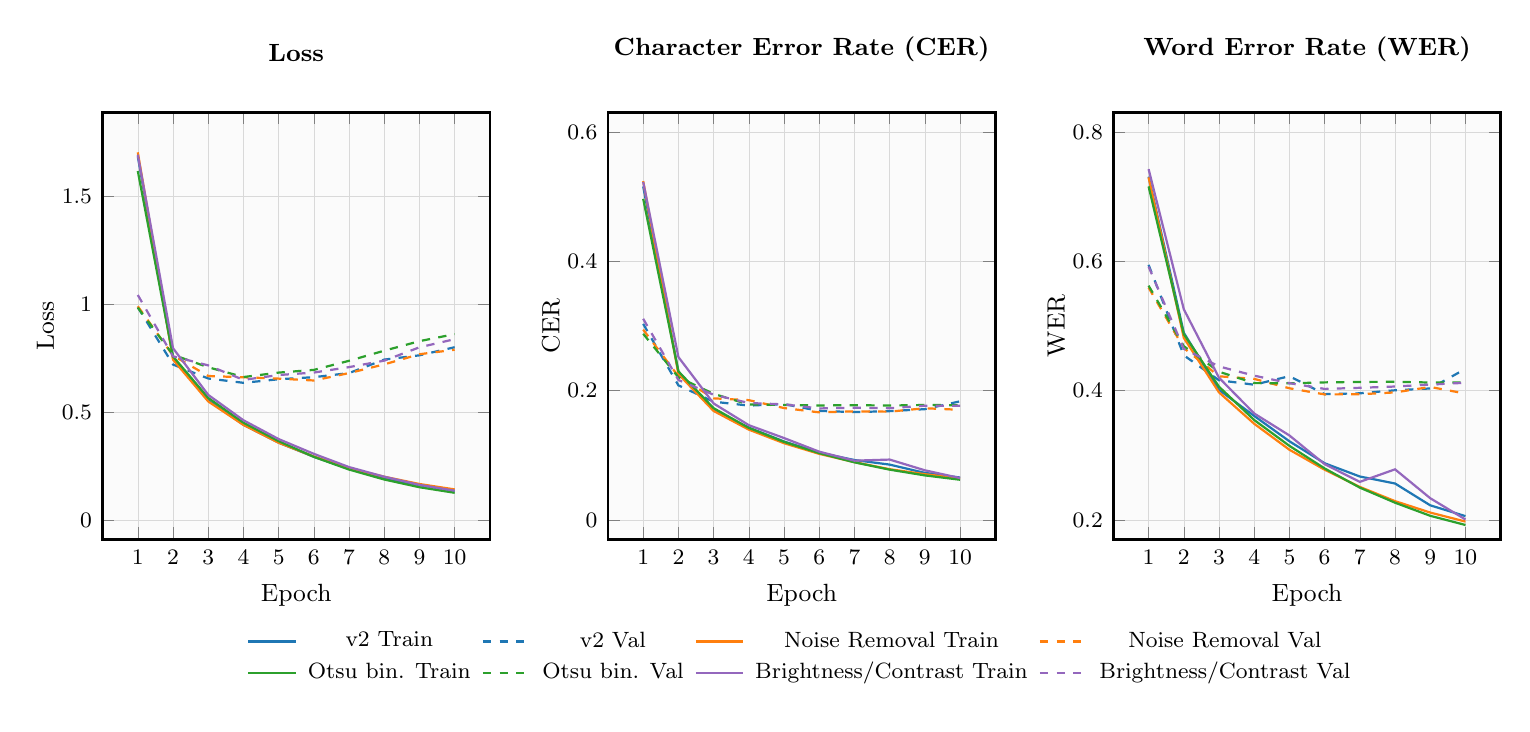
\begin{tikzpicture}[remember picture]

    % Graph 1: Loss
    \begin{axis}[
        name=plot1,
        width=6.5cm,
        height=7cm,
        xlabel={Epoch},
        ylabel={Loss},
        ylabel style={yshift=-0.15cm},
        xmin=0.5, xmax=10.5,
        ymin=0, ymax=1.8,
        xtick={1,2,3,4,5,6,7,8,9,10},
        grid=both,
        grid style={line width=.1pt, draw=gray!10},
        major grid style={line width=.2pt,draw=gray!30},
        title={Loss},
        axis background/.style={fill=gray!3},
        title style={yshift=3mm, font=\small\bfseries},
        label style={font=\small},
        tick label style={font=\footnotesize},
        line width=1pt,
        enlarge x limits=0.05,
        enlarge y limits=0.05,
        every axis plot/.append style={no markers},
        legend to name=commonlegend,
        legend columns=4,
        legend style={draw=none, fill=none, font=\footnotesize, column sep=2pt}
    ]
        % Original v2 Train
        \addplot[color=originalColor, thick] coordinates {
            (1, 1.6864) (2, 0.7533) (3, 0.5544) (4, 0.4414) (5, 0.3582)
            (6, 0.2928) (7, 0.2364) (8, 0.1938) (9, 0.1611) (10, 0.1348)
        };
        
        % Original v2 Validation
        \addplot[color=originalColor, thick, dashed] coordinates {
            (1, 0.9872) (2, 0.7209) (3, 0.6562) (4, 0.6361) (5, 0.6526)
            (6, 0.6623) (7, 0.6813) (8, 0.7440) (9, 0.7637) (10, 0.8013)
        };
        
        % Noise Removal Train (first 10 epochs)
        \addplot[color=noiseColor, thick] coordinates {
            (1, 1.7057) (2, 0.7435) (3, 0.5498) (4, 0.4408) (5, 0.3580)
            (6, 0.2943) (7, 0.2395) (8, 0.2003) (9, 0.1665) (10, 0.1414)
        };
        
        % Noise Removal Validation (first 10 epochs)
        \addplot[color=noiseColor, thick, dashed] coordinates {
            (1, 0.9914) (2, 0.7630) (3, 0.6677) (4, 0.6618) (5, 0.6556)
            (6, 0.6469) (7, 0.6813) (8, 0.7217) (9, 0.7688) (10, 0.7896)
        };
        
        % Otsu Train
        \addplot[color=otsuColor, thick] coordinates {
            (1, 1.6190) (2, 0.7584) (3, 0.5660) (4, 0.4509) (5, 0.3654)
            (6, 0.2924) (7, 0.2336) (8, 0.1873) (9, 0.1515) (10, 0.1257)
        };
        
        % Otsu Validation
        \addplot[color=otsuColor, thick, dashed] coordinates {
            (1, 0.9848) (2, 0.7662) (3, 0.7083) (4, 0.6629) (5, 0.6835)
            (6, 0.6961) (7, 0.7383) (8, 0.7852) (9, 0.8294) (10, 0.8621)
        };
        
        % Brightness/Contrast Train
        \addplot[color=brightColor, thick] coordinates {
            (1, 1.6949) (2, 0.7969) (3, 0.5801) (4, 0.4623) (5, 0.3750)
            (6, 0.3065) (7, 0.2450) (8, 0.2004) (9, 0.1625) (10, 0.1355)
        };
        
        % Brightness/Contrast Validation
        \addplot[color=brightColor, thick, dashed] coordinates {
            (1, 1.0436) (2, 0.7591) (3, 0.7170) (4, 0.6498) (5, 0.6722)
            (6, 0.6837) (7, 0.7090) (8, 0.7390) (9, 0.8009) (10, 0.8386)
        };
        
        \legend{v2 Train, v2 Val, Noise Removal Train, Noise Removal Val, Otsu bin. Train, Otsu bin. Val, Brightness/Contrast Train, Brightness/Contrast Val}
    \end{axis}
    
    % Graph 2: CER, positioned to the right of plot1
    \begin{axis}[
        name=plot2,
        at={($(plot1.east)+(1.5cm,0)$)},
        anchor=west,
        width=6.5cm,
        height=7cm,
        xlabel={Epoch},
        ylabel={CER},
        ylabel style={yshift=-0.15cm},
        xmin=0.5, xmax=10.5,
        ymin=0, ymax=0.6,
        xtick={1,2,3,4,5,6,7,8,9,10},
        grid=both,
        grid style={line width=.1pt, draw=gray!10},
        major grid style={line width=.2pt,draw=gray!30},
        title={Character Error Rate (CER)},
        axis background/.style={fill=gray!3},
        title style={yshift=3mm, font=\small\bfseries},
        label style={font=\small},
        tick label style={font=\footnotesize},
        line width=1pt,
        enlarge x limits=0.05,
        enlarge y limits=0.05,
        every axis plot/.append style={no markers}
    ]
        % Original v2 Train
        \addplot[color=originalColor, thick] coordinates {
            (1, 0.5158) (2, 0.2296) (3, 0.1693) (4, 0.1427) (5, 0.1213)
            (6, 0.1039) (7, 0.0926) (8, 0.0855) (9, 0.0727) (10, 0.0655)
        };
        
        % Original v2 Validation
        \addplot[color=originalColor, thick, dashed] coordinates {
            (1, 0.3032) (2, 0.2081) (3, 0.1828) (4, 0.1768) (5, 0.1791)
            (6, 0.1686) (7, 0.1667) (8, 0.1682) (9, 0.1713) (10, 0.1834)
        };
        
        % Noise Removal Train (first 10 epochs)
        \addplot[color=noiseColor, thick] coordinates {
            (1, 0.5240) (2, 0.2256) (3, 0.1685) (4, 0.1396) (5, 0.1186)
            (6, 0.1021) (7, 0.0893) (8, 0.0784) (9, 0.0707) (10, 0.0642)
        };
        
        % Noise Removal Validation (first 10 epochs)
        \addplot[color=noiseColor, thick, dashed] coordinates {
            (1, 0.2943) (2, 0.2221) (3, 0.1880) (4, 0.1852) (5, 0.1730)
            (6, 0.1663) (7, 0.1679) (8, 0.1674) (9, 0.1727) (10, 0.1703)
        };
        
        % Otsu Train
        \addplot[color=otsuColor, thick] coordinates {
            (1, 0.4966) (2, 0.2297) (3, 0.1728) (4, 0.1423) (5, 0.1206)
            (6, 0.1032) (7, 0.0890) (8, 0.0777) (9, 0.0688) (10, 0.0621)
        };
        
        % Otsu Validation
        \addplot[color=otsuColor, thick, dashed] coordinates {
            (1, 0.2879) (2, 0.2206) (3, 0.1950) (4, 0.1785) (5, 0.1779)
            (6, 0.1770) (7, 0.1774) (8, 0.1769) (9, 0.1777) (10, 0.1774)
        };
        
        % Brightness/Contrast Train
        \addplot[color=brightColor, thick] coordinates {
            (1, 0.5228) (2, 0.2519) (3, 0.1801) (4, 0.1465) (5, 0.1266)
            (6, 0.1055) (7, 0.0916) (8, 0.0933) (9, 0.0767) (10, 0.0647)
        };
        
        % Brightness/Contrast Validation
        \addplot[color=brightColor, thick, dashed] coordinates {
            (1, 0.3111) (2, 0.2164) (3, 0.1936) (4, 0.1808) (5, 0.1787)
            (6, 0.1724) (7, 0.1735) (8, 0.1728) (9, 0.1766) (10, 0.1767)
        };
    \end{axis}
    
    % Graph 3: WER, positioned to the right of plot2
    \begin{axis}[
        name=plot3,
        at={($(plot2.east)+(1.5cm,0)$)},
        anchor=west,
        width=6.5cm,
        height=7cm,
        xlabel={Epoch},
        ylabel={WER},
        ylabel style={yshift=-0.15cm},
        xmin=0.5, xmax=10.5,
        ymin=0.2, ymax=0.8,
        xtick={1,2,3,4,5,6,7,8,9,10},
        grid=both,
        grid style={line width=.1pt, draw=gray!10},
        major grid style={line width=.2pt,draw=gray!30},
        title={Word Error Rate (WER)},
        axis background/.style={fill=gray!3},
        title style={yshift=3mm, font=\small\bfseries},
        label style={font=\small},
        tick label style={font=\footnotesize},
        line width=1pt,
        enlarge x limits=0.05,
        enlarge y limits=0.05,
        every axis plot/.append style={no markers}
    ]
        % Original v2 Train
        \addplot[color=originalColor, thick] coordinates {
            (1, 0.7310) (2, 0.4895) (3, 0.4012) (4, 0.3608) (5, 0.3216)
            (6, 0.2876) (7, 0.2671) (8, 0.2563) (9, 0.2225) (10, 0.2058)
        };
        
        % Original v2 Validation
        \addplot[color=originalColor, thick, dashed] coordinates {
            (1, 0.5945) (2, 0.4546) (3, 0.4160) (4, 0.4091) (5, 0.4223)
            (6, 0.3945) (7, 0.3958) (8, 0.4005) (9, 0.4033) (10, 0.4336)
        };
        
        % Noise Removal Train (first 10 epochs)
        \addplot[color=noiseColor, thick] coordinates {
            (1, 0.7299) (2, 0.4816) (3, 0.3972) (4, 0.3487) (5, 0.3085)
            (6, 0.2776) (7, 0.2510) (8, 0.2290) (9, 0.2113) (10, 0.1974)
        };
        
        % Noise Removal Validation (first 10 epochs)
        \addplot[color=noiseColor, thick, dashed] coordinates {
            (1, 0.5593) (2, 0.4659) (3, 0.4221) (4, 0.4181) (5, 0.4036)
            (6, 0.3941) (7, 0.3943) (8, 0.3972) (9, 0.4056) (10, 0.3954)
        };
        
        % Otsu Train
        \addplot[color=otsuColor, thick] coordinates {
            (1, 0.7159) (2, 0.4874) (3, 0.4060) (4, 0.3545) (5, 0.3145)
            (6, 0.2796) (7, 0.2499) (8, 0.2266) (9, 0.2063) (10, 0.1921)
        };
        
        % Otsu Validation
        \addplot[color=otsuColor, thick, dashed] coordinates {
            (1, 0.5623) (2, 0.4687) (3, 0.4292) (4, 0.4116) (5, 0.4112)
            (6, 0.4127) (7, 0.4134) (8, 0.4136) (9, 0.4125) (10, 0.4124)
        };
        
        % Brightness/Contrast Train
        \addplot[color=brightColor, thick] coordinates {
            (1, 0.7427) (2, 0.5259) (3, 0.4199) (4, 0.3646) (5, 0.3306)
            (6, 0.2862) (7, 0.2588) (8, 0.2782) (9, 0.2335) (10, 0.2006)
        };
        
        % Brightness/Contrast Validation
        \addplot[color=brightColor, thick, dashed] coordinates {
            (1, 0.5918) (2, 0.4646) (3, 0.4374) (4, 0.4231) (5, 0.4115)
            (6, 0.4026) (7, 0.4043) (8, 0.4063) (9, 0.4094) (10, 0.4121)
        };
    \end{axis}

    % Positioning the common legend below all graphs
    \node at ($(plot1.south)!0.5!(plot3.south)+(0,-1.5cm)$) {\pgfplotslegendfromname{commonlegend}};
    
\end{tikzpicture}
\end{document}